\documentclass[conference]{IEEEtran}

\usepackage[T1]{fontenc}
\usepackage[utf8]{inputenc}
\usepackage{amsmath,amssymb,amsthm}
\usepackage{graphicx}
\usepackage{booktabs}
\usepackage{multirow}
\usepackage{xcolor}
\usepackage{colortbl}
\usepackage{listings}
\usepackage{tikz}
\usepackage{pgfplots}
\pgfplotsset{compat=1.18}
\usepackage{hyperref}
\usepackage{microtype}
\usepackage{balance}
\usetikzlibrary{shapes.geometric,arrows.meta,positioning,fit,backgrounds,calc}

\lstset{
  basicstyle=\ttfamily\scriptsize,
  breaklines=true,
  frame=single,
  rulecolor=\color{gray!30},
  backgroundcolor=\color{gray!5},
  numbers=left,
  numberstyle=\tiny\color{gray},
  numbersep=4pt,
  xleftmargin=8pt,
}

\title{WatchTower: Observation-First Forensics for Multi-Agent AI Systems\\
\large Detecting Silent Failures and Report-vs-Reality Gaps When an
Agent's Self-Report Is Not Ground Truth}

\author{\IEEEauthorblockN{Rohit Jinsiwale}
\IEEEauthorblockA{Proof-of-Concept Artifact\\
\url{https://github.com/beejak/agentwatch}}}

\begin{document}
\maketitle

\begin{abstract}
Monitoring tools for LLM-agent systems consume what an agent \emph{reports} it did---the
trace of tool calls and outputs it emits. We argue this is insufficient as a security signal:
agents fail in ways their self-report does not reveal, and a compromised or buggy agent (or
tool) can under-report its own actions. We characterize two structural blind spots---\emph{silent
failures} (the agent reports success while looping, burning tokens, or collapsing in output
diversity) and \emph{cross-layer discrepancies} (the agent's reported actions disagree with an
independent host view)---and present \textsc{WatchTower}, an observation-first platform that
detects them by reconciling the self-report against (a)~the \emph{shape} of the execution
trajectory and (b)~an independent \emph{host} ground truth. On a frozen, held-out corpus a
faithful self-report baseline detects \textbf{0\%} of both classes \emph{by construction},
while \textsc{WatchTower} detects silent failures at $0.86$ recall ($0.07$ FP) and cross-layer
discrepancies at $1.00$ ($0.00$ FP). We confirm the mechanism on \textbf{real, emergent
traffic} from an LLM agent whose behavior is captured through an egress proxy ($n{=}120$;
recall $1.00$, FP $0.00$), and we map the detection envelope---including where detection falls
off. This paper documents a proof-of-concept artifact released for reproduction and extension;
\textsc{WatchTower} observes and attributes but does not enforce (a co-designed enforcement
layer is described separately).
\end{abstract}

\section{Introduction}
LLM agents increasingly act through tools, memory, and peer agents. Existing observability
(LangSmith, Langfuse) records the agent's emitted trace and renders it on a dashboard. That
trace is the agent's \emph{self-report}, and a self-report is not ground truth:

\begin{itemize}
\item \textbf{The silent failure.} An agent retries the same call $150$ times; every span is
\texttt{status=ok}; cost balloons. Nothing \emph{errored}---an output-level monitor shows a
green dashboard while the task was broken throughout.
\item \textbf{The lying agent.} An agent's trace reports one network call; the host observed
four. The three unreported calls are invisible to anything that trusts the trace---an
exfiltration/tampering signal.
\end{itemize}

We argue monitoring must \emph{reconcile the self-report against independent evidence}---the
trajectory's shape and an independent host view---and that the discrepancy is the signal.

\noindent\textbf{Contributions.}
\begin{itemize}
\item \textbf{C1, silent-failure detection (SC2):} cost-anomaly, retry-loop, and
entropy-collapse detectors that flag failures which never raise an error.
\item \textbf{C2, cross-layer reconciliation (SC3):} comparison of agent-reported network
actions against host telemetry, scored as a tamper/exfil discrepancy.
\item \textbf{C3, an append-only forensic Chronicle + attribution (SC1):} a no-UPDATE/no-DELETE
event store enabling post-hoc attribution of a coordination failure to agent, action, and
call-tree position.
\item \textbf{Evidence:} a frozen, held-out evaluation with baselines and confidence intervals,
an operating-envelope sweep, and confirmation on real emergent LLM-agent traffic. All artifacts
are released for reproduction.
\end{itemize}

\section{Background and Related Work}
\textbf{Trace/output monitors} (LangSmith, Langfuse) record and visualize the emitted trace;
they trust the self-report and thus cannot flag an all-\texttt{ok} silent failure, nor detect a
report-vs-reality gap (no host concept). \textbf{The observability gap}~\cite{obsgap} argues
output-level feedback is insufficient for coding agents; we operationalize that argument with
concrete detectors and an evaluation. \textbf{Agentic process observability}~\cite{procobs}
treats trajectories as process-mining targets and highlights stochasticity; it is complementary,
not a security discrepancy detector. \textbf{Host EDR} (Sysmon, Falco, eBPF) observes OS-level
network/process events but has no agent semantics; \textsc{WatchTower} \emph{bridges} host events
to the agent trajectory via process GUIDs. The \textbf{MAST} taxonomy~\cite{mast} informs the
coordination-failure signatures used in attribution. Our novelty is \emph{multi-layer
reconciliation (self-report $\leftrightarrow$ trajectory $\leftrightarrow$ host) as a security
signal}, with concrete detectors, a forensic substrate, and a held-out evaluation.

\section{Threat and Failure Model}
We consider agents that may report success while failing---non-adversarial bugs (retry storms,
token burn) and adversarial masking---and a compromised/injected agent (or tool) that
under-reports network activity (SC3 exfil). \emph{In scope:} detection, attribution, forensic
record. \emph{Out of scope (companion enforcement system):} blocking, prompt-injection content
classification, and cross-session taint.

\section{System Design}
\textsc{WatchTower} is a passive, append-only, 16-layer side-car (Fig.~\ref{fig:pipeline}).
Agents emit HMAC-signed \texttt{Signal}s to a Redis stream; a Receiver verifies origin on every
signal and fans out to inspection layers; everything is recorded to an append-only
\textbf{Chronicle} (ClickHouse; no UPDATE/DELETE; 90-day TTL). Analyses run over the Chronicle.

\begin{figure}[t]
\centering
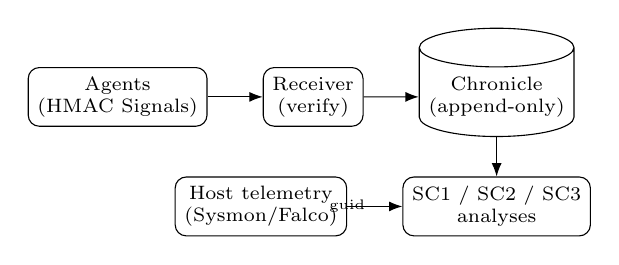
\begin{tikzpicture}[
  node distance=5mm and 7mm, >=Latex,
  box/.style={draw, rounded corners, align=center, font=\scriptsize, minimum height=6mm},
  db/.style={draw, cylinder, shape border rotate=90, aspect=0.25, align=center, font=\scriptsize}]
\node[box] (a) {Agents\\(HMAC Signals)};
\node[box, right=of a] (r) {Receiver\\(verify)};
\node[db, right=of r] (c) {Chronicle\\(append-only)};
\node[box, below=of c] (an) {SC1 / SC2 / SC3\\analyses};
\node[box, left=of an] (h) {Host telemetry\\(Sysmon/Falco)};
\draw[->] (a)--(r); \draw[->] (r)--(c); \draw[->] (c)--(an);
\draw[->] (h)-- node[font=\tiny,left]{guid} (an);
\end{tikzpicture}
\caption{Observe-and-reconcile pipeline. The Chronicle is the forensic source of truth;
SC3 reconciles the agent self-report against host telemetry by process GUID.}
\label{fig:pipeline}
\end{figure}

\noindent\textbf{SC1 attribution.} From a trace's spans, identify the failing agent/action and
call-tree position, classified against a coordination-signature (MAST) library.

\noindent\textbf{SC2 silent failure.} Over a trace's spans: a cost-anomaly ratio
(actual/expected), a repeated-summary retry-loop test, and an entropy-collapse test---none of
which require an error status.

\noindent\textbf{SC3 cross-layer.} Count agent-reported network actions; count host
\texttt{NetworkConnect} events for the same process GUIDs; a positive delta (host $>$ reported)
is the discrepancy.

A three-stage verdict engine (deterministic $\rightarrow$ behavioral-baseline $\rightarrow$
sampled LLM judge) and a per-agent behavioral baseline ($3\sigma$; restricted until $50$ traces)
support the analyses.

\section{Implementation}
Python~3.12 (all-async), Pydantic~v2 (the \texttt{Signal} shape defined once), a FastAPI
surface, a ClickHouse Chronicle, Redis transport, PostgreSQL baseline, Neo4j access graph,
HMAC-SHA256 signing, and 12-factor environment configuration. A lightweight SDK lets any agent
emit signed signals to the Chronicle or the \texttt{wt:signals} stream. Approximately 16 layers,
each gated by a test. The LLM judge is a real OpenAI-compatible client when configured, and a
deterministic heuristic otherwise---so the pipeline and CI run with zero LLM dependency.

\section{Evaluation}
We use frozen, human-labeled corpora; a held-out split; baselines head-to-head; and bootstrap
$95\%$ confidence intervals. Baselines: \textbf{B1} self-report (flags only an explicit error
span---the faithful upper bound of any self-report-trusting monitor) and \textbf{B2} a naive
cost threshold. All numbers are reproducible from the released artifacts: the synthetic corpus
is \texttt{eval/corpus/traces\_v0.1.jsonl} (results \texttt{eval/results/traces\_v0.1\_test.json});
the real-LLM corpus \texttt{eval/corpus/captured\_llm\_v0.1.jsonl}
(\texttt{eval/results/captured\_llm\_test.json}); the envelope sweep
\texttt{eval/results/sweep\_v0.1.json}.

\begin{table}[t]
\caption{Held-out synthetic corpus ($n{=}269$; 380-trace corpus).}
\label{tab:synth}
\centering\footnotesize
\begin{tabular}{lcccc}
\toprule
Detector & SC2 recall & SC2 FPR & SC3 recall & SC3 FPR \\
\midrule
\textbf{WatchTower} & \textbf{0.86} & 0.07 & \textbf{1.00} & 0.00 \\
Self-report (B1)    & 0.00 & 0.00 & 0.00 & 0.00 \\
Naive cost (B2)     & 0.27 & 0.07 & --- & --- \\
\bottomrule
\end{tabular}
\end{table}

\noindent\textbf{H3 (the spine).} The self-report baseline has \textbf{0 recall} on both
classes---it never sees the signal (Fig.~\ref{fig:recall}). \textsc{WatchTower} also beats naive
cost (loops/entropy catch what pure cost misses; pure cost false-positives on
expensive-but-correct work).

\begin{figure}[t]
\centering
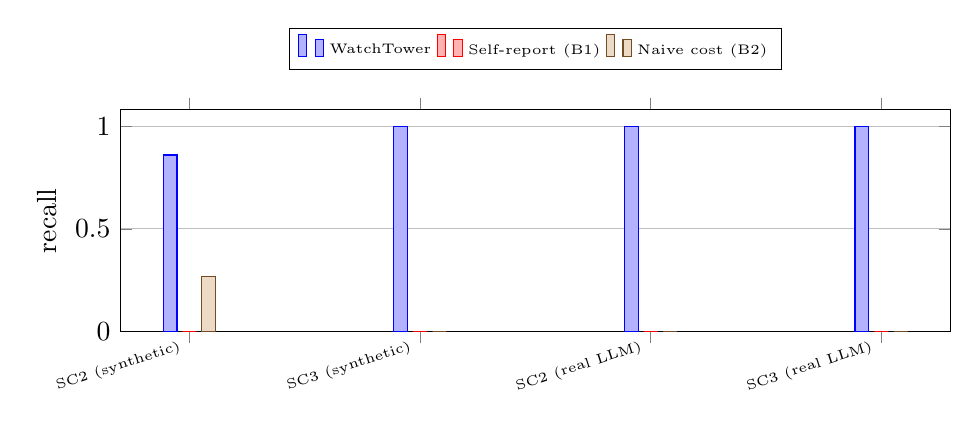
\begin{tikzpicture}
\begin{axis}[
  ybar, width=\columnwidth, height=4.4cm, ymin=0, ymax=1.08,
  ylabel={recall}, symbolic x coords={SC2 (synthetic),SC3 (synthetic),SC2 (real LLM),SC3 (real LLM)},
  xtick=data, x tick label style={rotate=18,anchor=east,font=\tiny}, bar width=5pt,
  ymajorgrids, legend style={font=\tiny,at={(0.5,1.18)},anchor=south,legend columns=3}]
\addplot coordinates {(SC2 (synthetic),0.86) (SC3 (synthetic),1.00) (SC2 (real LLM),1.00) (SC3 (real LLM),1.00)};
\addplot coordinates {(SC2 (synthetic),0.00) (SC3 (synthetic),0.00) (SC2 (real LLM),0.00) (SC3 (real LLM),0.00)};
\addplot coordinates {(SC2 (synthetic),0.27) (SC3 (synthetic),0.00) (SC2 (real LLM),0.00) (SC3 (real LLM),0.00)};
\legend{WatchTower, Self-report (B1), Naive cost (B2)}
\end{axis}
\end{tikzpicture}
\caption{Detection recall by detector, on held-out synthetic and real LLM-driven traffic.
\textbf{H3:} the self-report baseline is structurally blind ($0.00$) across the board, while
\textsc{WatchTower} detects.}
\label{fig:recall}
\end{figure}

\begin{table}[t]
\caption{Operating envelope---where detection holds and falls off.}
\label{tab:env}
\centering\footnotesize
\begin{tabular}{ll}
\toprule
Condition & Boundary \\
\midrule
SC2 silent loop & fires at loop length $\geq 10$ (shorter missed) \\
SC2 token burn  & fires at total cost $\geq \$0.12$ (FP above on costly-OK) \\
SC3 cross-layer & fires at delta $\geq 1$; negative delta never fires \\
SC1 attribution & $0.50$: cascade exposes first-error $\neq$ causal-root \\
\bottomrule
\end{tabular}
\end{table}

\begin{figure}[t]
\centering
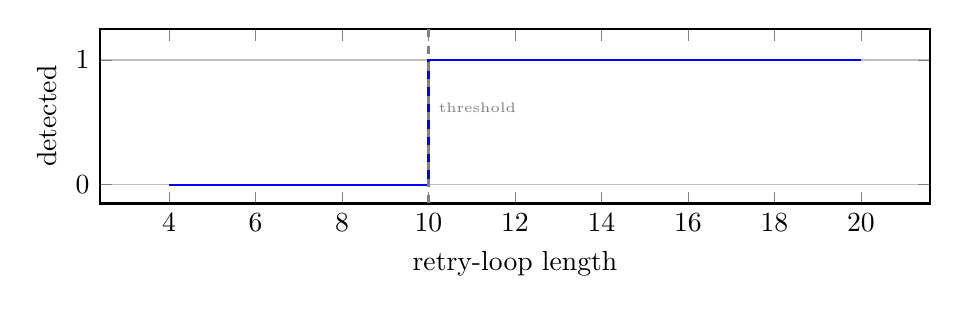
\begin{tikzpicture}
\begin{axis}[
  width=\columnwidth, height=3.8cm, ymin=-0.15, ymax=1.25,
  xlabel={retry-loop length}, ylabel={detected}, ytick={0,1},
  xtick={4,6,8,10,12,14,16,18,20}, ymajorgrids, const plot, thick]
\addplot+[mark=none] coordinates {(4,0)(6,0)(8,0)(9,0)(10,1)(12,1)(16,1)(20,1)};
\draw[dashed,gray] (axis cs:10,-0.15)--(axis cs:10,1.25);
\node[font=\tiny,gray,anchor=south west] at (axis cs:10,0.5) {threshold};
\end{axis}
\end{tikzpicture}
\caption{SC2 operating envelope: silent-loop detection turns on at loop length $\geq 10$
(shorter loops are honest misses). Token-burn fires at cost $\geq\$0.12$; SC3 fires at
host$-$reported delta $\geq 1$ (negative delta---telemetry sampling---never fires).}
\label{fig:env}
\end{figure}

\begin{table}[t]
\caption{Near-real-world: real LLM agent, emergent traffic ($n{=}120$, 40/class).}
\label{tab:llm}
\centering\footnotesize
\begin{tabular}{lcccc}
\toprule
Detector & SC2 recall & SC2 FPR & SC3 recall & SC3 FPR \\
\midrule
\textbf{WatchTower} & \textbf{1.00} & 0.00 & \textbf{1.00} & 0.00 \\
Self-report (B1)    & 0.00 & 0.00 & 0.00 & 0.00 \\
\bottomrule
\end{tabular}
\end{table}

\noindent\textbf{Near-real-world methodology.} A DeepSeek agent (ReAct loop) acts against tasks;
its tools make real HTTP egress through an independent egress proxy (mitmproxy) that records
every call regardless of whether the agent emitted a span. SC2 (the model genuinely loops) and
SC3 (a compromised tool's hidden egress) \emph{emerge} from the model's behavior---nothing is
scripted. Table~\ref{tab:llm} confirms H3 on real traffic. The $1.00$ reflects a clean signal
once the condition occurs; the conservative headline is the synthetic $0.86$ of
Table~\ref{tab:synth}, which includes borderline cases.

\section{Discussion and Limitations}
\begin{itemize}
\item \textbf{Attribution is first-error, not causal-root.} On cascade failures where the root
error is not the first error span, SC1 mis-identifies the agent (Table~\ref{tab:env}).
Causal-root attribution is future work.
\item \textbf{Synthetic realism.} The bulk corpus is generated; the robust result is the
structural \emph{baseline gap}, confirmed on real LLM-agent traffic. Absolute numbers will move
on production traffic.
\item \textbf{SC3 without kernel telemetry} validates HTTP egress only (proxy); raw-socket, DNS,
and proxy-bypass require an eBPF/Sysmon collector (a bridge is implemented and unit-tested).
\item \textbf{Captured scale.} The real-agent corpus is $120$ traces---ample to confirm the
mechanism, modest for headline claims; the harness scales with a parameter.
\item \textbf{LLM judge is fallible}---it is the last, sampled verdict stage by design;
deterministic stages are authoritative.
\end{itemize}

\section{Conclusion}
Treating an agent's self-report as untrusted---and reconciling it against the trajectory and an
independent host view---catches silent failures and report-vs-reality gaps that
self-report-based monitoring structurally cannot. We release the implementation, frozen
corpora, and harness as a proof-of-concept artifact for reproduction and extension.

\section*{Artifact Availability}
All code, frozen corpora, results, and this paper are released at
\url{https://github.com/beejak/agentwatch}. Reproduce: \texttt{make eval} (held-out synthetic,
Table~\ref{tab:synth}), \texttt{python -m eval.sweep} (operating envelope, Table~\ref{tab:env}
and Fig.~\ref{fig:env}), and \texttt{make capture-tier1-llm} (real LLM-driven capture,
Table~\ref{tab:llm}). Data: \texttt{eval/corpus/traces\_v0.1.jsonl} ($n{=}380$) and
\texttt{eval/corpus/captured\_llm\_v0.1.jsonl} ($n{=}120$); per-run metrics in
\texttt{eval/results/*.json}; end-to-end demo output in \texttt{examples/sample\_output.json};
methodology in \texttt{docs/TESTING.md} and \texttt{docs/REAL\_TRAFFIC\_VALIDATION.md}. The
companion enforcement system is at \url{https://github.com/beejak/agentwatch-firewall}.

\begin{thebibliography}{9}
\bibitem{obsgap} ``The Observability Gap in LLM Coding Agents,'' arXiv:2603.26942, 2026.
\bibitem{procobs} ``Agentic AI Process Observability,'' arXiv:2505.20127, 2025.
\bibitem{mast} Cohen et al., ``MAST: A Multi-Agent System Taxonomy for LLM Failure Mode
Classification,'' NeurIPS, 2025.
\bibitem{owasp} OWASP, ``Top 10 for LLM Applications,'' 2025.
\bibitem{sysmon} Microsoft, ``Sysmon,'' Sysinternals; Falco, ``Cloud-native runtime security.''
\end{thebibliography}

\balance
\end{document}
